\documentclass[11pt]{article}
\usepackage{amsmath, amssymb}
\usepackage{geometry}
\geometry{margin=1in}
\usepackage{fancyhdr}
\usepackage{lastpage}
\usepackage{parskip} % Better paragraph spacing
\usepackage{titlesec} % Better section formatting
\usepackage{graphicx}
\usepackage{float}
\usepackage[most]{tcolorbox}
\usepackage{lmodern}
\usepackage{caption}
\usepackage{hyperref}
\usepackage{listings}
\usepackage{xcolor}

\definecolor{codegreen}{rgb}{0,0.6,0}
\definecolor{codegray}{rgb}{0.5,0.5,0.5}
\definecolor{codepurple}{rgb}{0.58,0,0.82}
\definecolor{backcolour}{rgb}{0.95,0.95,0.92}

% Define code styling
\lstdefinestyle{mystyle}{
    backgroundcolor=\color{backcolour},
    commentstyle=\color{codegreen},
    keywordstyle=\color{magenta},
    numberstyle=\tiny\color{codegray},
    stringstyle=\color{codepurple},
    basicstyle=\ttfamily\footnotesize,
    breakatwhitespace=false,
    breaklines=true,
    captionpos=b,
    keepspaces=true,
    numbers=left,
    numbersep=5pt,
    showspaces=false,
    showstringspaces=false,
    showtabs=false,
    tabsize=2
}

\lstset{style=mystyle}

% Define commands for reusable content
\newcommand{\coursename}{CS-401 Applied Data Analysis}
\newcommand{\lecturenum}{09}
\newcommand{\lecturedate}{12/11/2025}
\newcommand{\professor}{Maria Brbic}

\hypersetup{colorlinks=true,linkcolor=blue,urlcolor=blue}

% Configure section spacing
\titlespacing*{\section}{0pt}{2ex plus 1ex minus .2ex}{1.5ex plus .2ex}
\titlespacing*{\subsection}{0pt}{1.5ex plus 1ex minus .2ex}{1ex plus .2ex}
% Header / Footer
\pagestyle{fancy}
\fancyhf{}
\fancyhead[L]{\coursename}
\fancyhead[R]{Lecture \lecturenum}
\fancyfoot[L]{EPFL - Computer Science}
\fancyfoot[C]{Author: Jonathan Dutoit}
\fancyfoot[R]{Page \thepage\ of \pageref{LastPage}}

\begin{document}

\begin{center}
  {\large EPFL - Computer Science} \\[0.5em]
  {\Large \textbf{\coursename}} \\[0.5em]
  {\large Lecture \lecturenum\ --- \lecturedate} \\[0.5em]
  {\large Author: Jonathan Dutoit} \\[0.5em]
  {\large Professor: \professor} \\[0.5em]
\end{center}

\vspace{2cm}

\begin{center}
  {\LARGE \textbf{Unsupervised Learning}}
\end{center}

\vspace{1cm}

\textbf{\textcolor{red}{Unsupervised}}: Given only samples \textit{X} of the data, we compute a function f such that \textcolor{blue}{\textit{y = f(X)}} is a "simpler" representation:
\begin{itemize}
	\item \textcolor{orange}{Discrete} \textit{y} (cluster labels): \textbf{"clustering"}
	\item \textcolor{green}{Continuous} \textit{y}" \textbf{\textcolor{blue}{"dimensionality reduction"}} \textcolor{blue}{e.g., matrix factorization, unsupervised neural networks)}
\end{itemize}

\section*{The clustering problem}

\begin{itemize}
	\item Given a \textcolor{purple}{set of points}, with a notion of \textcolor{purple}{distance} between points, \textcolor{purple}{group the points} into some number of \textit{\textbf{\textcolor{green}{clusters}}}, such that 
		\begin{itemize}
			\item members of a cluster are close (i.e., similar) to each other
			\item members of different clusters are far apart from each other
		\end{itemize}
	\item \textbf{\textcolor{red}{Usually}}:
		\begin{itemize}
			\item Points live in a high-dimensional space
			\item Similarity is defined via a distance measure (Euclidean cosine, Jaccard, edit distance ...)
		\end{itemize}
\end{itemize}

\section*{Characteristics of clustering methods}

Clustering algorithms have the following properties: 

\textbf{\textcolor{purple}{Quantitative}}: scalability (many samples), dimensionality (many features)

\textbf{\textcolor{orange}{Qualitative}}: types of features (numerical, categorical, etc.), type of shapes (polyhedra, hyperplanes, manifolds, etc.)

\textbf{\textcolor{green}{Robustness}}: sensitivity to noise and outliers, sensitivity to the processing order

\textbf{\textcolor{blue}{User interaction}}: incorporation of user constraints (e.g., number of clusters, max size of clusters), interpretability and usability. 

\newpage
\section*{Some use cases for clustering}

\begin{itemize}
	\item Data exploration (especially for high-dimensional data, where visualization fails)
	\item Partitioning of data for more fine-grained subsequent analysis
	\item Marking: building personas
	\item Supporting data labeling for supervised learning
	\item Supporting feature discretization for supervised learning
	\item Data compression
	\item ...
\end{itemize}

\section*{Clustering for condensation/compression}

% Quick centered image
\begin{figure}[H]
    \centering
    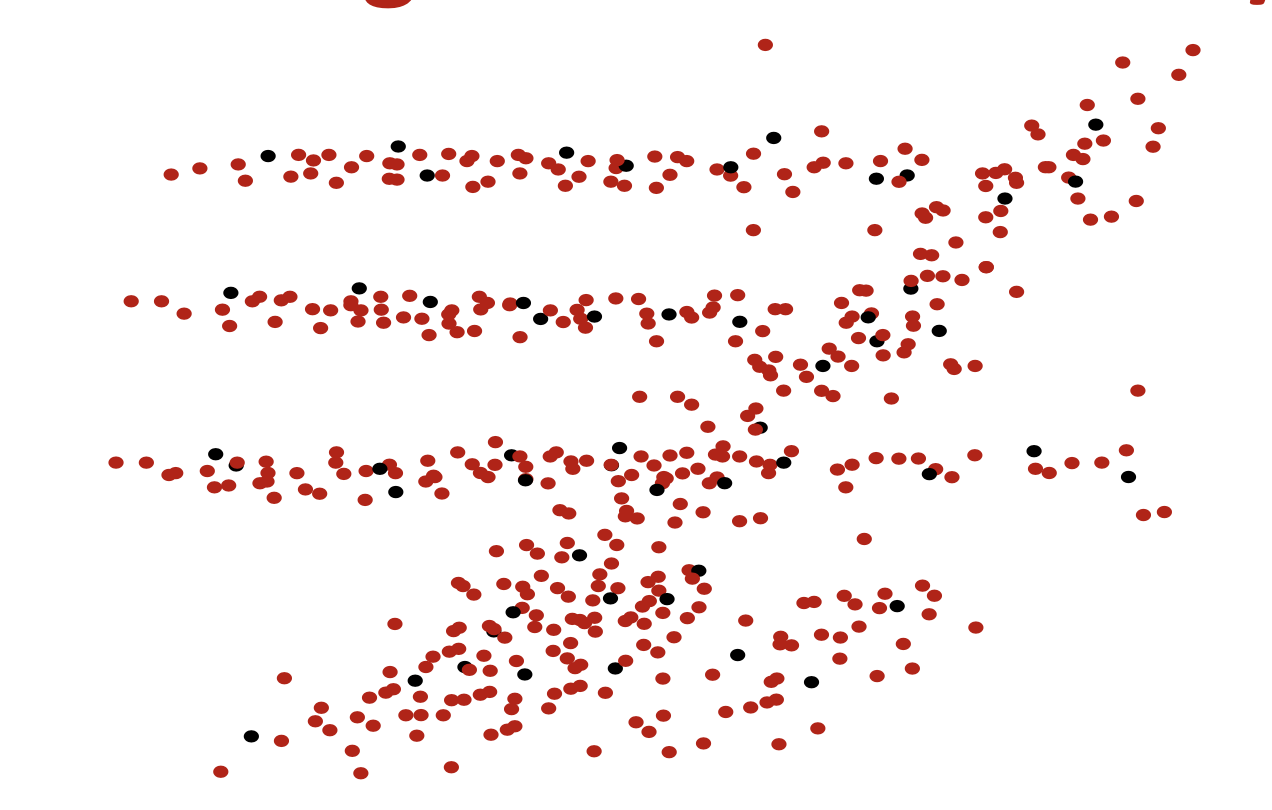
\includegraphics[width=0.6\textwidth]{compression}
    \label{fig:LABEL}
\end{figure}

In the picture above, the black dots are "class representatives" of the data. We don't require that clusters extract meaningful structure, but that they give a coarse-grained version of the data. 

\section*{Beware of "cluster bias"!}

\begin{itemize}
	\item Human beings conceptualize the world through categories represented as exemplars or prototypes
	\item We tend to see cluster structure whether it is there or not.
	\item Works well for dogs, but...
\end{itemize}

% Quick centered image
\begin{figure}[H]
    \centering
    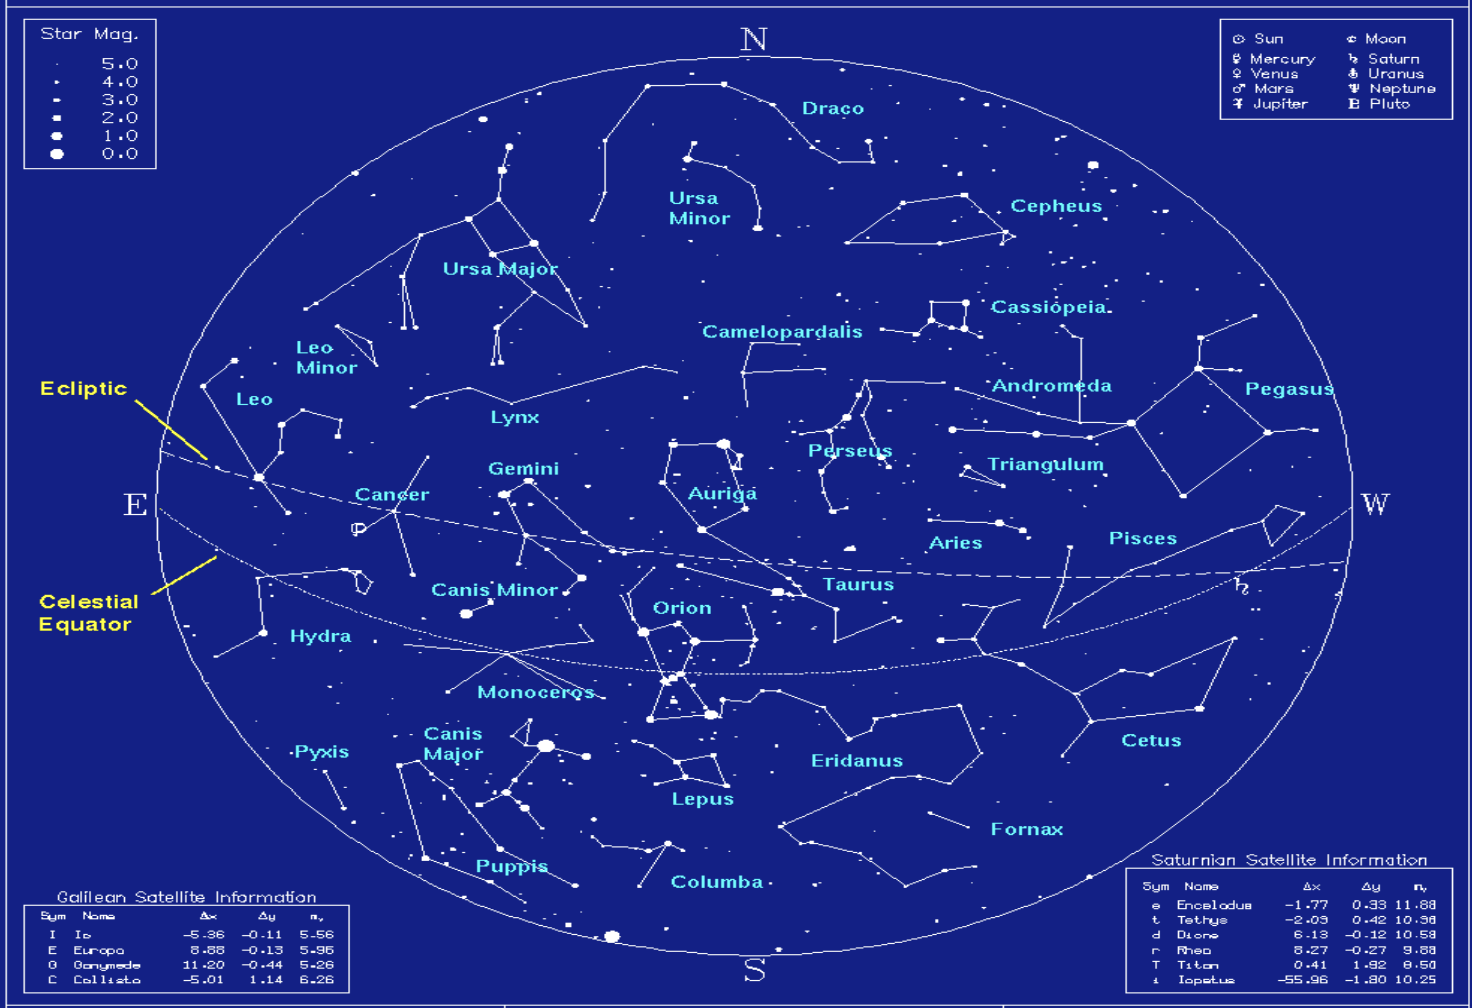
\includegraphics[width=0.8\textwidth]{stars}
    \label{fig:LABEL}
\end{figure}

Even if we see structures/figures, it doesn't mean that statistically it makes sense. 

\section*{Cluster bias}

\begin{itemize}
	\item \textbf{\textcolor{orange}{Clustering is used more than it should be}}, because people assume an underlying domain has discrete classes in it
		\begin{itemize}
			\item Especially true for characteristics of people, e.g., Myers-Briggs personality types like "ENTP". 
		\end{itemize}
	\item In reality the underlying data is often \textbf{\textcolor{red}{continuous}}
	\item In such cases, continuous models (e.g., matrix factorization, "soft" clustering where we use probabilities) tend to do beter
\end{itemize}

% Quick centered image
\begin{figure}[H]
    \centering
    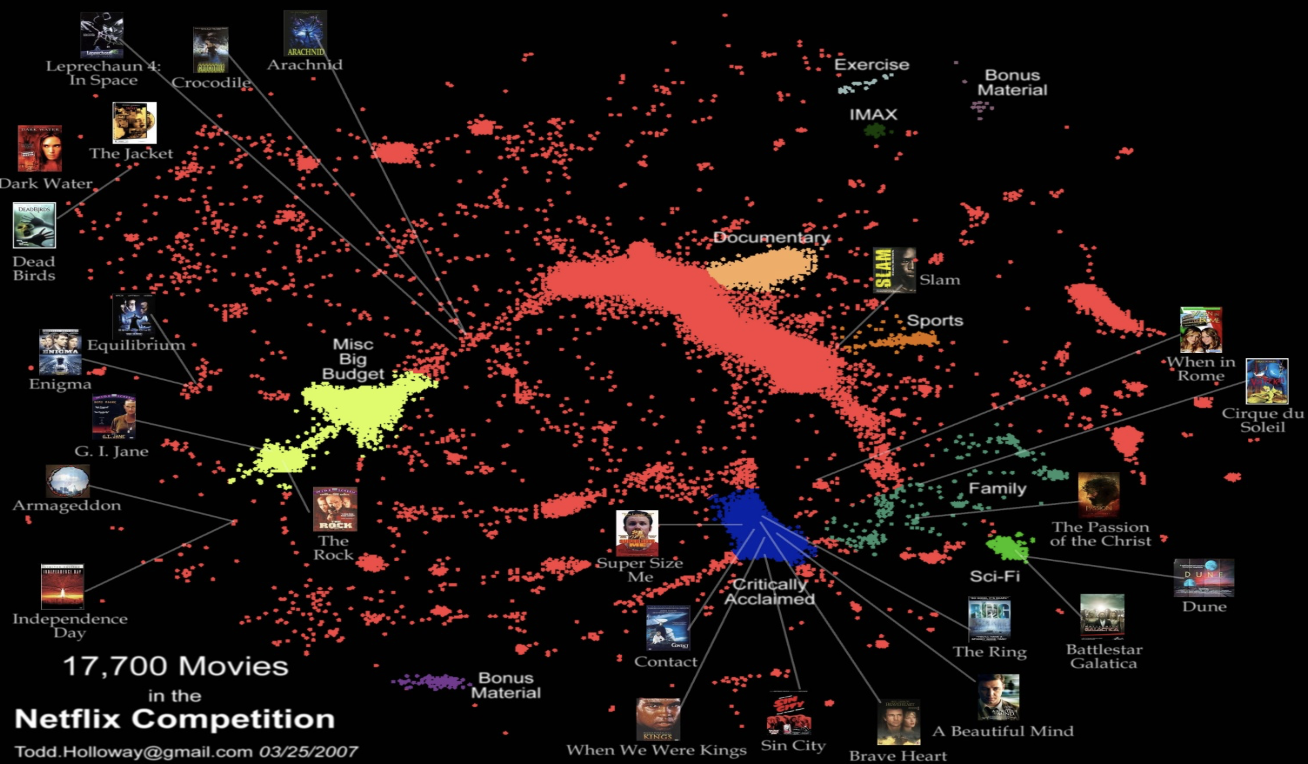
\includegraphics[width=0.7\textwidth]{netflix}
    \label{fig:LABEL}
\end{figure}

In this Netflix dataset, each data point is a movie that is represented by a vector of real numbers based on user's watching it or not. There are million of users, hence this was dimensionality reduce to be able to see it in 2D. 

Note that the closer movies are in this space, the more similar they are too. 

\begin{itemize}
	\item Central portion: more of a continuum than discrete cluster
	\item Other methods (e.g., dimensionality reduction) may be more appropriate than discrete clustering methods.
\end{itemize}

\section*{Terminology}

\begin{itemize}
	\item \textcolor{blue}{Hierarchical clustering}: cluster form a tree-shaped hierarchy. Can be computed bottom-up or top-down
	\item \textcolor{blue}{Flat clustering}: no inter-cluster structure
	\item \textcolor{orange}{Hard clustering}: items assigned to a unique cluster
	\item \textcolor{orange}{Soft clustering}: cluster membership is a probability distribution over all clusters
\end{itemize}

\section*{Clustering is hard}
\begin{itemize}
	\item Clustering small amounts of data (like 2 dimensions) looks easy, and actually is often easy but...
	\item ... many applications involve not 2, but hundreds or thousands of dimensions (and large amounts of data)
	\item High-dimensional spaces are different ("\textit{\textbf{curse of dimensionality}}"): volume grows exponentially with the number of dimensions; space is sparsely populated; clusters become less tight. 
\end{itemize}

\section*{Clustering problem: galaxies}

\begin{itemize}
	\item A catalog of 2 billion "sky objects" represents objects by their radiation in 7 dimensions (frequency bands)
	\item Problem: cluster into similar objects, e.g., galaxies, nearby stars, quasars, etc. 
	\item Sloan Digital Sky Survey
\end{itemize}

\section*{Clustering problem: movies}

\begin{itemize}
	\item \textbf{Intuitively: Movies divide into categories/genres, and customers prefer a few categories}
		\begin{itemize}
			\item But what are categories really? 
			\item $\Rightarrow$ take a data-driven approach!
		\end{itemize}
	\item Represents a movie by a set of customers who watched it ("collaborative filtering")
	\item \textbf{Idea}: Similar movies have similar sets of customers, and vice-versa
\end{itemize}

\textbf{Space of all movies}:
\begin{itemize}
	\item Think of a space with one dimension for each customer
		\begin{itemize}
			\item Values in a dimension may be 0 or 1 only
			\item A movie is a point in this space $(x_1, x_2, ..., x_n)$ where $x_i$ = 1 iff the \textit{i}=th customer watched the movie
		\end{itemize}
	\item For Amazon/Netflix, the dimensionality is in the millions
	\item \textbf{Task}: Find clusters of similar movies
\end{itemize}


\section*{Cosine, Jaccard, Euclidean distances}

In all examples, we have a choice when thinking of data points as sets of features:
\begin{itemize}
	\item Sets as vectors
		\begin{itemize}
			\item Measure similarity via \textbf{Euclidian distance} or \textbf{cosine distance}
		\end{itemize}
	\item Sets as sets:
		\begin{itemize}
			\item Measure similarity via \textbf{Jaccard index}
		\end{itemize}
\end{itemize}

\section*{Overview: Methods of clustering}

\textbf{\textcolor{blue}{Hierarchical methods:}}"
\begin{itemize}
	\item \textbf{Agglomerative} (bottom-up):
		\begin{itemize}
			\item Initially, each point is a cluster
	\item Repeatedly combine two "nearest" clusters into one
	\end{itemize}
		
	\item \textbf{Divisive} (top-down):
		\begin{itemize}
			\item Start with one cluster and recursively split it
		\end{itemize}
\end{itemize}

\textbf{\textcolor{orange}{Flat methods (a.k.a point-assignment methods):}}
\begin{itemize}
	\item Maintain a set of clusters
	\item Assign points to "nearest" cluster; recompute clusters; repeat
\end{itemize}

\subsection*{Agglomerative hierarchical clustering}

\vspace{0.25cm}
\textbf{Key operation}: repeatedly combine two nearest clusters

\textbf{Three important questions}:
\begin{itemize}
	\item (1) How to represent a cluster of more than one point?
		\begin{itemize}
			\item Euclidean case: represent a cluster via its \textbf{centroid} = average of points in cluster
			\item What about non-Euclidean case? 
		\end{itemize}
	\item (2) How to determine the "nearness" of clusters?
		\begin{itemize}
			\item Euclidean case: distance between clusters = distance between centroids
			\item What about non-Euclidean case?
		\end{itemize}
	\item (3) When to stop combining clusters?
\end{itemize}

\section*{Non-Euclidean case: clustroids}

(1) Howe to represent a cluster of many points?

\textbf{clustroid} = actual data point that is \textbf{"closest"} to the other points

\begin{itemize}
	\item Possible meanings of "closest" 
		\begin{itemize}
			\item Smallest average distance to other points (a.k.a \textbf{medoid})
			\item Smallest sum of squares of distances to other points
			\item Smallest maximum distance to other points
		\end{itemize}
\end{itemize}

\begin{minipage}{0.4\textwidth}

\textcolor{blue}{\textbf{Centroid} is the average of all data points in the cluster. This means centroid is an "artificial" point} \\

\textcolor{purple}{\textbf{clustroid} is an \textbf{existing} data point that is "closest" to all other points in the cluster.}
\end{minipage}
\hfill
\begin{minipage}{0.5\textwidth}
\centering
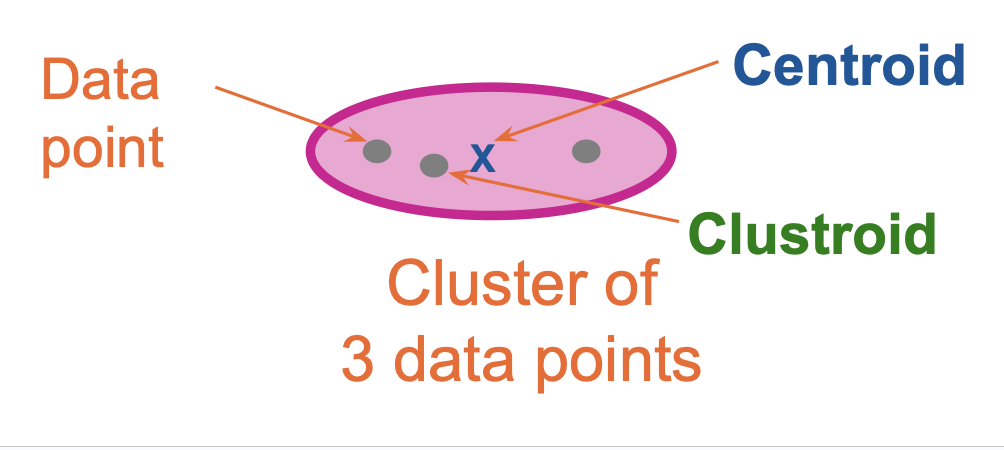
\includegraphics[width=\linewidth]{clustroid}
\end{minipage}


(2) How do you determine the "nearness" of clusters?
\begin{itemize}
	\item \textcolor{green}{Approach 1:} \\
	\textbf{Intercluster distance} = minimum of the distances between any two points, one from each cluster; or average of distances; or distance between clustroids; etc. 
	\item \textcolor{purple}{Approach 2:} \\
	Pick a notion of "\textbf{cohesion}" ("tightness") of a cluster \\
	Then: nearness of clusters = cohesion of their \textit{union}
\end{itemize}

\section*{Cohesion}

\begin{itemize}
	\item \textcolor{purple}{\textbf{Approach 2.1}}: Use the \textbf{diameter} of the merged cluster = maximum distance between points in the merged cluster
	\item \textcolor{purple}{\textbf{Approach 2.2}}: Use the \textbf{average distance} between points in the merged cluster
\end{itemize}

\section*{Implementation}

\begin{itemize}
	\item \textbf{Naïve implementation of hierarchical clustering}:
		\begin{itemize}
			\item At each step, compute pairwise distance between all pairs of clusters, then merge
			\item O($N^{3}$), where \textit{N} is the number of data points
		\end{itemize}
	\item \textbf{Careful implementation using priority queue} can reduce time to O($N^{2} \log{N}$)
		\begin{itemize}
			\item Still too expensive for really big datasets
		\end{itemize}
\end{itemize}

\newpage

\begin{center}
  {\LARGE \textbf{K-means}}
\end{center}
\vspace{0.5cm}

\textbf{Goal}: assign each data point to one of \textit{k} clusters such that the total distance of points to their centroids is minimized

\begin{itemize}
	\item Solved by a simple greedy algorithm (Lloyd's algorithm): \\
	Locally minimize the "distance" (usually squared Euclidean distance) from data points to their respective centroids:
	\begin{itemize}
		\item \textbf{\textcolor{orange}{Find the closest cluster centroid}} for each data point, and assign the point to that cluster
		\item \textbf{\textcolor{green}{Recompute the cluster centroid}} (the mean of data points in the cluster) for each cluster. 
	\end{itemize}
\end{itemize}

% Quick centered image
\begin{figure}[H]
    \centering
    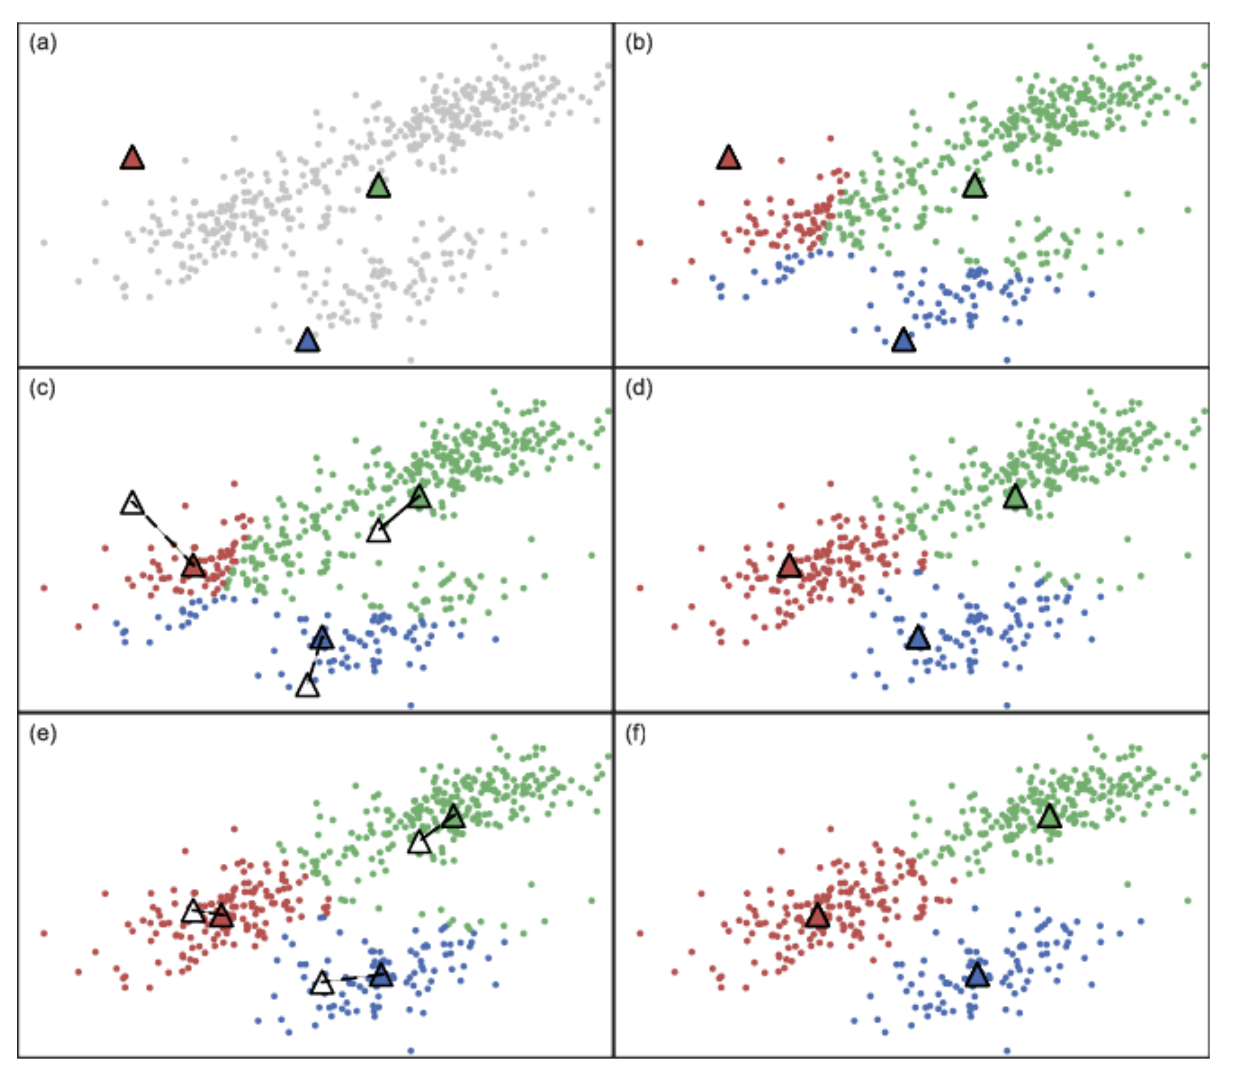
\includegraphics[width=0.8\textwidth]{k-means}
    \label{fig:LABEL}
\end{figure}

\textbf{\textcolor{red}{How long to iterate?}}
\begin{itemize}
	\item For fixed number of iterations
	\item or until no change in assignments (guaranteed to happen)
	\item or until only small change in cluster "tightness" (sum of [squared] distances from points to centroids)
\end{itemize}

\subsection*{K-means initialization}
We need to pick some points for the first round of the algorithm: 
\begin{itemize}
	\item \textcolor{red}{\textbf{Random sample}}: Pick a random subset of \textit{k} points from the dataset.
	\item \textcolor{red}{\textbf{K-Means++}}: Iteratively construct a random sample with good spacing across the dataset. 
\end{itemize}

\textbf{\textcolor{red}{Note}}: Finding an optimal k-means clustering is NP-hard. The above help avoid bad configurations. K-means is a \textbf{greedy algorithm}. 

\subsection*{K-means++}

\textbf{\textcolor{blue}{Start}}: Choose first cluster center at random from the data points

\textbf{\textcolor{blue}{Iterate}}: 
\begin{itemize}
	\item For every remaining data point \textit{x}, compute the distance \textit{D(x)} from \textit{x} to the closest previously selected cluster center. 
	\item Choose a remaining point \textit{x} randomly with probability proportional to $D(x)^{2}$, and make it a new cluster center. 
\end{itemize}

Intuitively, this finds a sample of widely-spaced points from dense regions of the data space, avoiding "collapsing" of the clustering into a few internal centers. 

\section*{K-means properties}

\begin{itemize}
	\item Greedy algorithm with random initialization - \textbf{\textcolor{red}{solution may be suboptimal}} and vary significantly with different initial points
	\item Very simple convergence proofs
	\item \textbf{\textcolor{red}{Performance is \textit{O(nk)} per iteration}} - not bad, and ca be heuristically improved. \\
		\textit{n} = number of points in the dataset, \textit{k} = number clusters
	\item Many variants, e.g., Fixed-size clusters, soft clustering
	\item Works well for data condensation/compression
\end{itemize}

\subsection*{K-means drawbacks}

Often terminates at \textbf{\textcolor{purple}{local but non-global optimum}} (mitigated by smart initialization such k-means++, or by re-running multiple times with different initializations)

Requires the notion of a \textbf{\textcolor{red}{mean}}

Requires specifying \textit{\textcolor{blue}{\textbf{k}}} (number of clusters) in advance

Doesn't handle \textbf{\textcolor{red}{noisy data and outliers}} well

Clusters \textbf{\textcolor{green}{only}} have \textbf{\textcolor{green}{convex shapes}}

% Quick centered image
\begin{figure}[H]
    \centering
    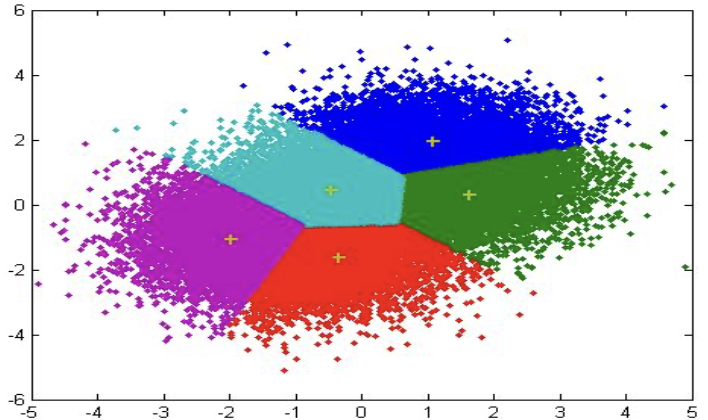
\includegraphics[width=0.8\textwidth]{convex}
    \label{fig:LABEL}
\end{figure}

\subsection*{How to choose number of clusters k?}

For k = 1, 2, 3, ...
\begin{itemize}
	\item Run k-means with \textit{k} clusters
	\item For each data point \textit{i}, compute "\textcolor{blue}{silhouette width}"
		\[
			s(i) = \frac{b(i) - a(i)}{max\{ a(i), b(i)\}}
		.\] 
		where \textit{b(i)}: avg. distance to points in closest other cluster, and \textit{a(i)}: avg. distance to points in own cluster
	\item S = average of \textit{s(i)} over all \textit{i}
	\item Plot S against \textit{k}
	\item Pick \textit{k} which S is greatest 
\end{itemize}

% Quick centered image
\begin{figure}[H]
    \centering
    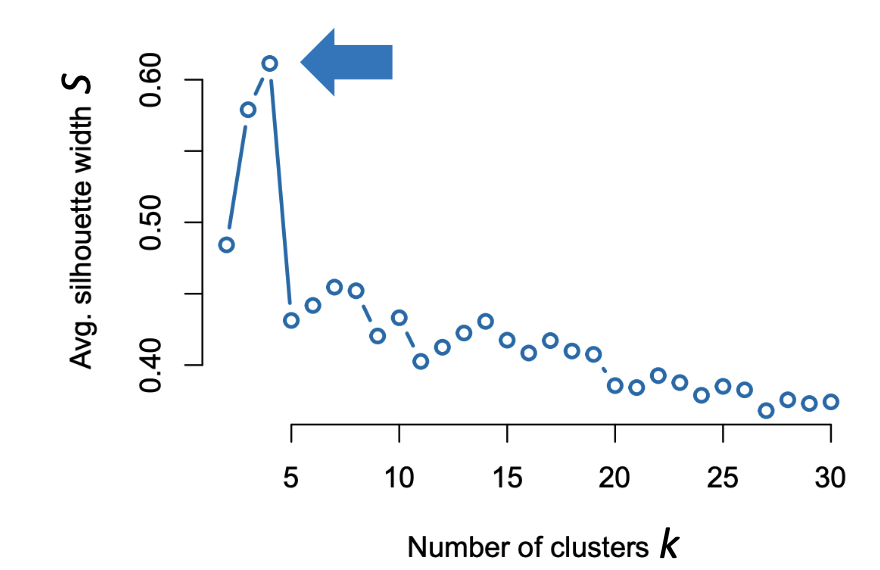
\includegraphics[width=0.6\textwidth]{choosing-k}
    \label{fig:LABEL}
\end{figure}

\section*{DBSCAN}

"\textcolor{red}{D}ensity-\textcolor{red}{b}ased \textcolor{red}{s}patial \textcolor{red}{c}lustering of \textcolor{red}{a}pplications with \textcolor{red}{n}oise"

\textbf{Motivation}: centroid-based clustering methods like k-means favor clusters that are spherical, and have great difficulty with anything else 

DBSCAN performs density-based clustering, and follows the shape of dense neighborhoods of pints. 

% Quick centered image
\begin{figure}[H]
    \centering
    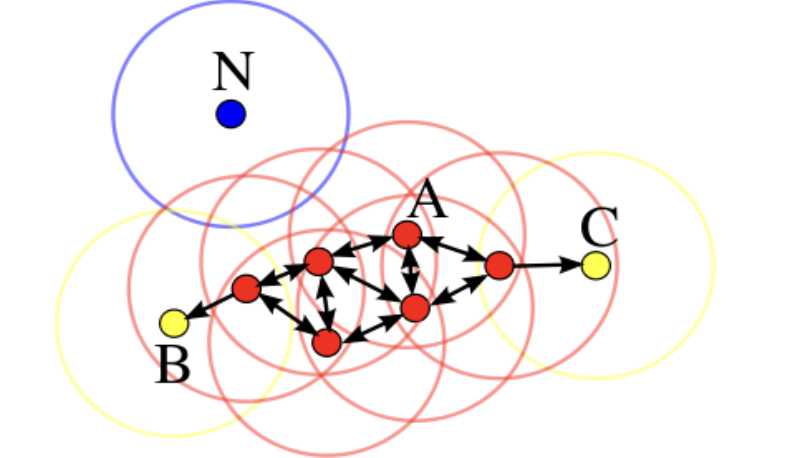
\includegraphics[width=0.5\textwidth]{dbscan}
    \label{fig:LABEL}
\end{figure}

\begin{itemize}
	\item \textbf{Def.:} \textbf{\textcolor{red}{core points}} have a lest \textit{minPts} neighbors in a sphere of diameter $\epsilon$ around them.
	\item The \textbf{\textcolor{red}{red}} points here are core points with at least \textit{minPts} = 3 neighbors in an $\epsilon$-sphere around them. 
\end{itemize}

\begin{itemize}
	\item \textcolor{red}{Core points} can \textbf{\textcolor{red}{directly reach}} neighbors in their $\epsilon$-sphere 
	\item From non-core points, no other points can be reached
	\item Points \textit{q} is \textbf{\textcolor{red}{density-reachable}} from \textit{p} if there is a series of points \textit{p} = $p_1, ..., p_n = q$ such that $p_{i+1}$ is directly reachable from $p_i$ (yellow points)
	\item All points not density-reachable from any other points are \textbf{\textcolor{blue}{outliers/noise}} (blue points)
	\item Points \textit{p, q} are \textbf{\textcolor{red}{density-connected}} if there is a point \textit{o} such that both \textit{p} and \textit{q} are density-reachable from \textit{o}.
	\item A \textcolor{red}{\textbf{cluster}} is a set of points that are \textbf{\textcolor{red}{mutually density-connected}}.
	\item That is, if a point is density-reachable from a cluster point, it is part of the cluster as well
	\item In the above figure, \textcolor{red}{red points} are mutually density-reachable; \textcolor{yellow}{B and C} are density-connected; \textcolor{blue}{N} is an outlier. 
\end{itemize}

\subsection*{DBSCAN performance}
\begin{itemize}
	\item DBSCAN uses all-pairs point distances, but using an efficient indexing structure, each RangeQuery (for finding neighbors within $\epsilon$-sphere) takes only $O(\log{n})$ time
	\item The algorithm overall can be made to run in \textcolor{red}{$O(n \log{n})$}
	\item Fast neighbor search becomes progressively harder (higher constants) in higher dimensions, due to the \textbf{curse of dimensionality}!
\end{itemize}



\end{document}
